\begin{figure}
    \centering
    \begin{subfigure}[t]{.47\textwidth}
        \centering
        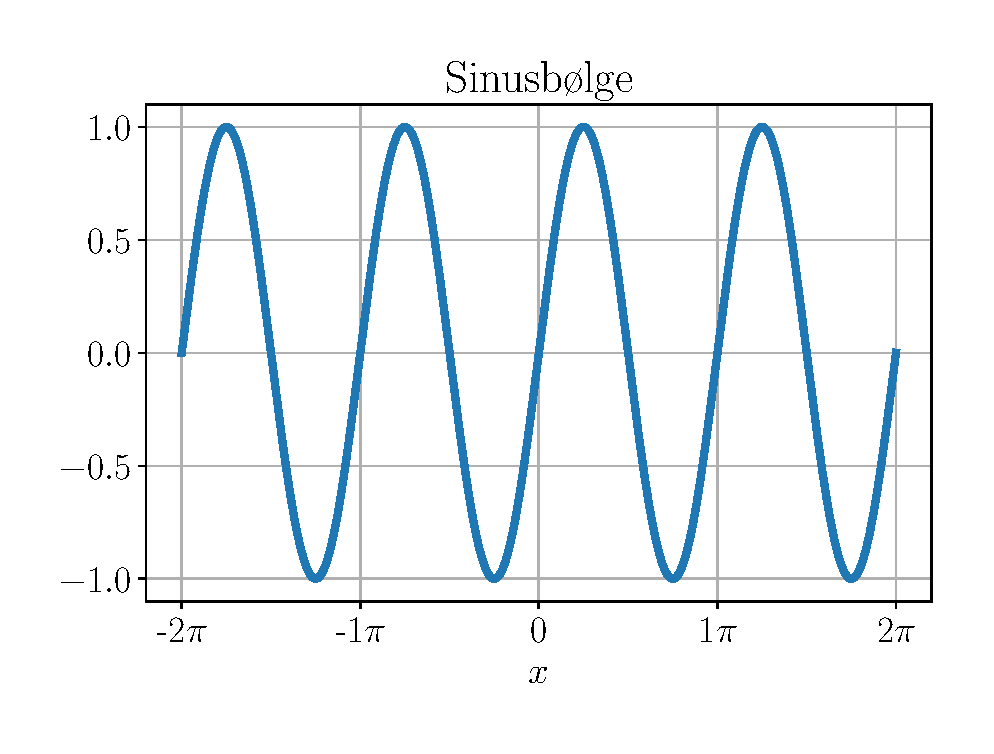
\includegraphics[width=\columnwidth]{Akustik/fig/sine_wave.eps}
        \caption{Sinusbølge, der udbreder sig i hele rummet.}
        \label{aku:fig:sine_wave}
    \end{subfigure}
    %
    \hfill
    %
    \begin{subfigure}[t]{.47\textwidth}
        \centering
        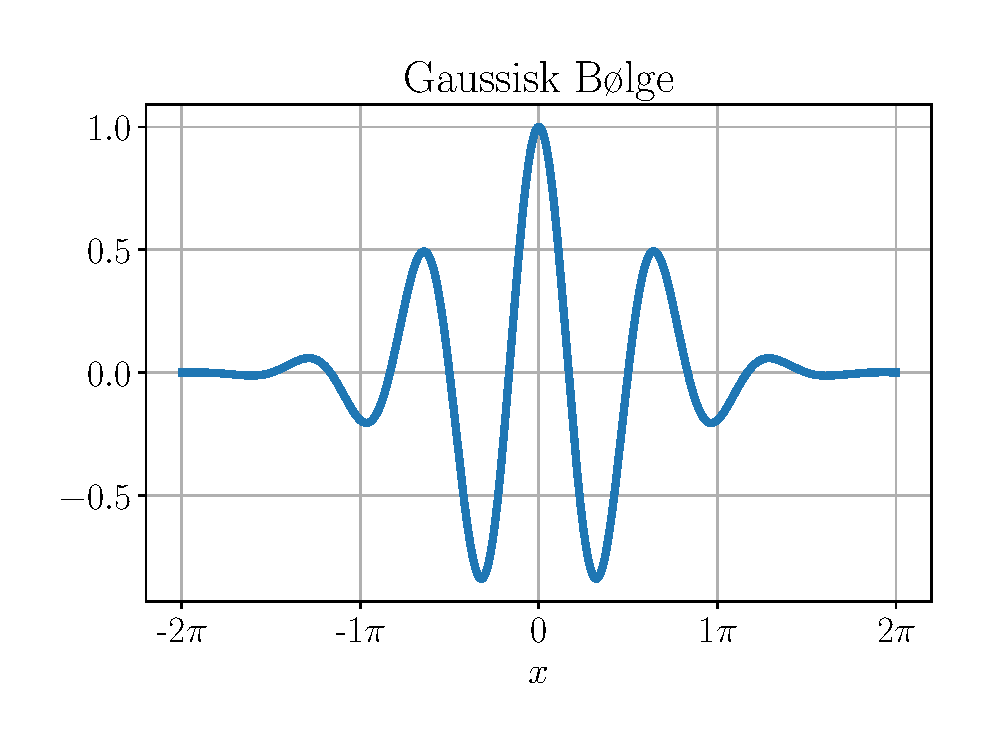
\includegraphics[width=\columnwidth]{Akustik/fig/gaussian_wave.eps}
        \caption{Gaussisk bølge, der er lokaliseret til et bestemt sted i rummet.}
        \label{aku:fig:gauss_wave}
    \end{subfigure}
    \caption{Eksempler på to forskellige typer bølger.}
    \label{aku:fig:wave}
\end{figure}

\section{Hvorfor er lyd bølger?} \label{aku:sec:wave}
For at kunne svare på dette spørgsmål fra Newtons love, skal man have en matematisk definition af hvad der menes med en bølge. Ofte siger man, at bølger er beskrevet ved sinus- og cosinusfunktioner, som den i \cref{aku:fig:sine_wave}. På \cref{aku:fig:gauss_wave} ses noget, der ikke er en sinusfunktion, men ikke desto mindre er en bølge. Matematisk set er bølger derfor mere end blot sinusbølger, men hvad definerer så en bølge? I fysik defineres en bølge, som en funktion, $f(x,t)$, der er en løsning til \textit{bølgeligningen}:
%
\begin{align} \label{aku:eq:wave}
    \pdv[2]{f(x,t)}{t} = v_\mathrm{lyd}^2\pdv[2]{f(x,t)}{x},
\end{align}
%
hvilket er en differentialligning. I \cref{aku:eq:wave} er $v_\mathrm{lyd}$ bølgens hastighed, $x$ er et stedkoordinat, $t$ er tid og $f(x,t)$ er en funktion af tid og sted, der beskriver bølgen. Løsningen til bølgeligningen er alle funktioner på formen $f(x\pm v_\mathrm{lyd}t)$. Kaldes funktionsargumentet $y$, således at $y = x \pm v_\mathrm{lyd}t$, fås ved brug af kædereglen at
%
\begin{subequations}
\begin{align}
    \pdv[2]{f(x\pm v_\mathrm{lyd}t)}{x} &= \pdv{f(y)}{y}\left(\pdv{f(y)}{y}\pdv{y}{x}\right) = \pdv[2]{f(y)}{y}\left(\pdv{y}{x}\right)^2 = \pdv[2]{f(y))}{y}, \label{aku:eq:wave_x}\\
    \pdv[2]{f(x\pm v_\mathrm{lyd}t)}{t} &= \pdv{f(y)}{y}\left(\pdv{f(y)}{y}\pdv{y}{t}\right) = \pdv[2]{f(y)}{y}\left(\pdv{y}{t}\right)^2 = v_\mathrm{lyd}^2\pdv[2]{f(y)}{y}, \label{aku:eq:wave_t}
\end{align}
\end{subequations}
%
idet $\partial^2y/\partial x^2 = \partial^2y/\partial t^2 = 0$. Sættes \cref{aku:eq:wave_x,aku:eq:wave_t} ind i \cref{aku:eq:wave} ses det, at funktioner på formen $f(x\pm v_\mathrm{lyd}t)$ er en løsning til bølgeligningen. Bølgens hastighed er $v_\mathrm{lyd}$, da funktioner på formen $f(x\pm v_\mathrm{lyd}t)$ svarer til at tage funktionen $f(x)$ og flytte nulpunktet fra $x_0=0$ til $x_0=\mp v_{lyd}t$. Differentieres nulpunktets bevægelsesligning fås $\nicefrac{\dd x_0}{\dd t} = \mp v_{lyd}$. Bølgens hastighed kaldes også gruppehastigheden, mens $\nicefrac{\dd f(x,t)}{\dd t}$ kaldes fasehastigheden, der beskriver hvor hurtigt punktet $x$ bevæger sig. Forskellen på gruppehastighed og fasehastighed er ikke vigtig for vores formål, hvorfor vi ikke gør mere ud af det, men den er vigtig i andre felter, der bruger bølgelære, som fx. optik. Vores formål er nu, at vise at lyd opfylder bølgeligningen. Vi vil undersøge en streng, eksempelvis fra en violin, og vise at når den vibrerer, så gør den det på en måde, der opfylder \cref{aku:eq:wave}. Til det formål skal Newtons anden lov skrives om til en form, der gælder for en streng, og ikke for en punktpartikel, som i \cref{mat:eq:N2}, hvorefter der skal opstilles en model for kraften på snoren.

\begin{figure}[t]
    \centering
    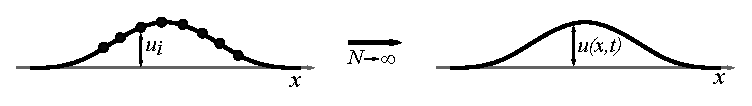
\includegraphics[width=\textwidth]{Akustik/fig/kontinuum.eps}
    \caption{Snoren beskrives som bestående af $N$ partikler med ens masse i grænsen hvor $N\rightarrow\infty$.}
    \label{aku:fig:kontinuum}
\end{figure}
\subsection{Kontinuummekanik}
I musikinstrumenter, der laver deres lyd gennem strenge, er strengen spændt op således at den danner en ret linje i rummet, hvilket er opspændte snores hviletilstand\footnote{Hviletilstanden kaldes også ligevægtstilstanden og er den tilstand snoren, hvor snoren står stille, ligesom en bold står stille i bunden af en bakkedal.}. Hvis snoren bestod af $N$ partikler, der var forbundet med masseløse snore, så ville man beskrive hver partikel med en stedfunktion $u_i(t)$, der fortæller hvor langt den $i$'te partikel er fra sin hvileposition. Acceleration ville så være bestemt af Newtons anden lov som $a_i = F_i/m_i$. Her er $F_i$ summen af snorkrafter, der virker på den $i$'te partikel, og $m_i = m/N$, hvor $m$ er massen af hele snoren, således at massen af snoren er summen af partiklernes masser. Problemet ved denne beskrivelse er snoren i virkeligheden er kontinuert -- den består ikke at individuelle partikler forbundet af snore -- og Newtons anden lov kan derfor ikke bruges til at beskrive snorens vibrationer. For at beskrive snoren som værende kontinuert, skal man betragte grænsen $N \rightarrow \infty$, hvilket kaldes kontinuitetsgrænsen\footnote{Formalistisk set skal vi introducere det, der hedder klassisk feltteori, hvor snoren beskrives som et éndimensionelt felt, der udvikler sig i tid, eller et todimensionel felt i rum og tid, hvis man vil være konsistent med speciel relativitetsteori. Hvis man også kræver, at feltet skal opfylde kvantemekanik, fås kvantefeltteori, der er den teori, som bruges i partikelfysik og så vidt muligt også kernefysik. I kvantefeltteori har bølgeligningen et særligt navn, hvor den er et særtilfælde af Klein-Gordon-ligningen, der beskriver masseløse partikler uden spin, der dog ikke er observeret eksperimentelt.}. Snoren beskrives altså som bestående af uendeligt mange infinitesimale\footnote{Med andre ord uendeligt små.} stykker, hvilket er illustreret i \cref{aku:fig:kontinuum}. I denne grænse beskriver man derfor snoren med én funktion, $u(x,t)$, der fortæller, hvor langt væk fra hvile snoren er ved stedkoordinatet $x$. Derudover beskrives snorens masse ved en massetæthed, $\mu(x)$, der defineres således at $m = \int_0^L\mu(x)\dd{x}$, hvor $L$ er snores længde. For et infinitesimalt stykke af snoren er massetætheden konstant, hvorfor
%
\begin{align}
    m_i = \int_x^{x+\Delta x}\mu\dd{x'} = \mu\int_x^{x+\Delta x}\dd{x'} = \mu\Delta x.
\end{align}
%
I \cref{sec:matematik} blev acceleration defineret i \cref{mat:eq:acceleration} som
%
\begin{align} \label{aku:eq:accelleration}
    a = \dv[2]{u(x,t)}{t}.
\end{align}
%
Ligning \eqref{aku:eq:accelleration} indeholder en totalafledede mht. tid, så derfor skal man overveje hvilke parametre, der kan afhænge af tiden. $u(x,t)$ afhænger af tiden $t$ og stedet $x$, hvor $t$ oplagt afhænger af $t$. Hvis $x$ afhænger af tiden, så betyder det, at det koordinatsystem, som snoren beskrives i, ændrer sig med tiden. Vi vælger et koordinatsystem, der er fastholdt i tid\footnote{Helt præcist betyder det at $\nicefrac{\dd{x}}{\dd{t}} = 0$, hvilket den interesserede læser vha. kædereglen kan vise medfører at $\nicefrac{\dd{u}}{\dd{t}} = \nicefrac{\partial u}{\partial t}$.}, hvilket betyder at $\nicefrac{\dd{u}}{\dd{t}} = \nicefrac{\partial u}{\partial t}$, hvorfor
%
\begin{align}
    a = \dv[2]{u(x,t)}{t} = \pdv[2]{u(x,t)}{t}.
\end{align}
%
Vi har således vist at man i kontinuitetsgrænsen får
%
\begin{align} \label{aku:eq:n2_kin}
    m_ia_i \xrightarrow[]{N\rightarrow\infty} \mu\Delta x \pdv[2]{u(x,t)}{t},
\end{align}
%
hvilket af Newtons anden lov skal være lig med kraften på delelementet.

\begin{figure}
    \begin{subfigure}[t]{.675\textwidth}
        \centering
        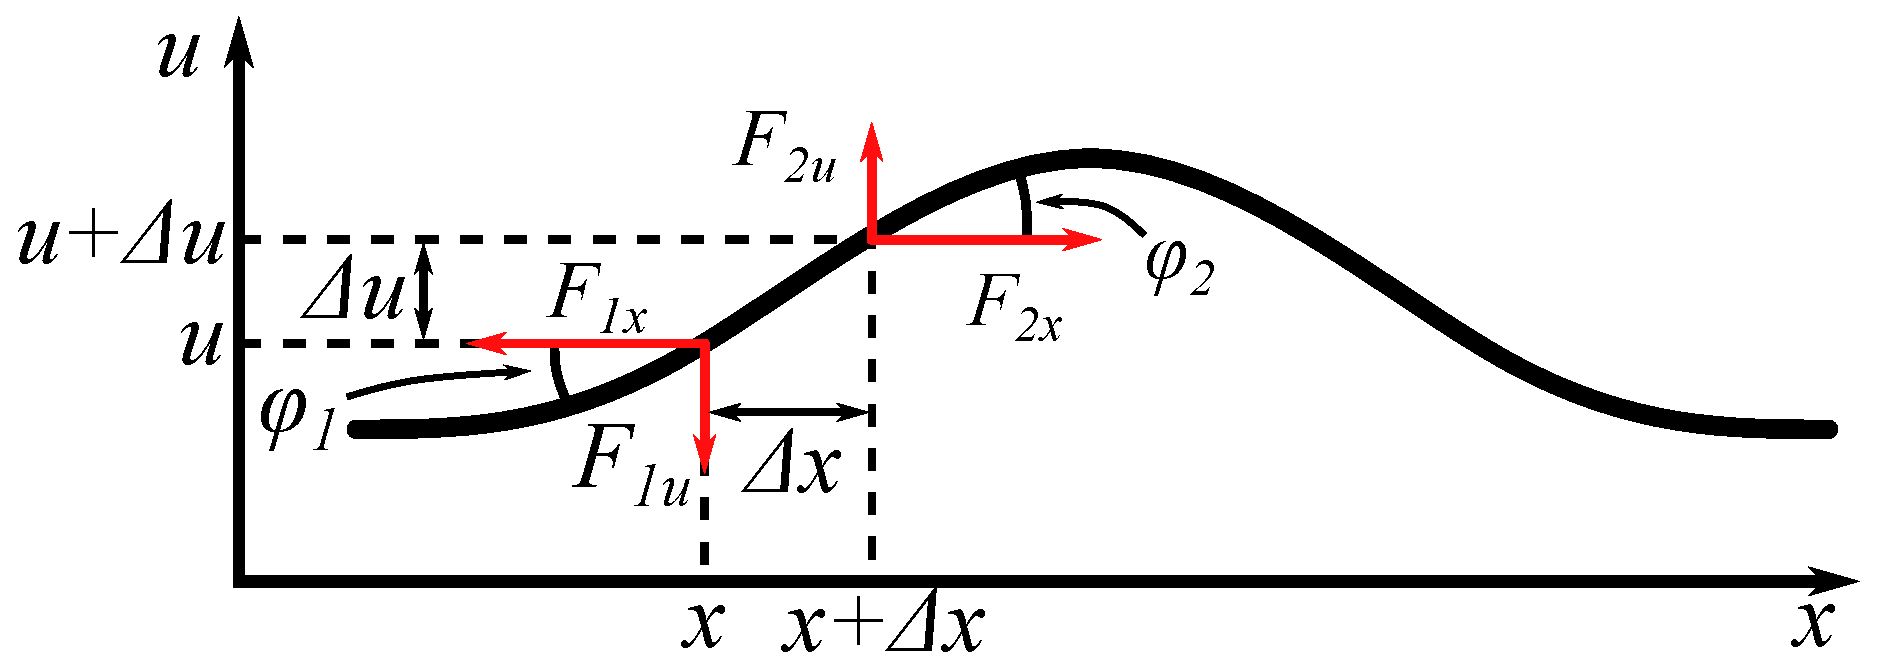
\includegraphics[width=\columnwidth]{Akustik/fig/snor.eps}
    \end{subfigure}
    %
    \hfill
    %
    \begin{subfigure}[t]{.225\textwidth}
        \centering
        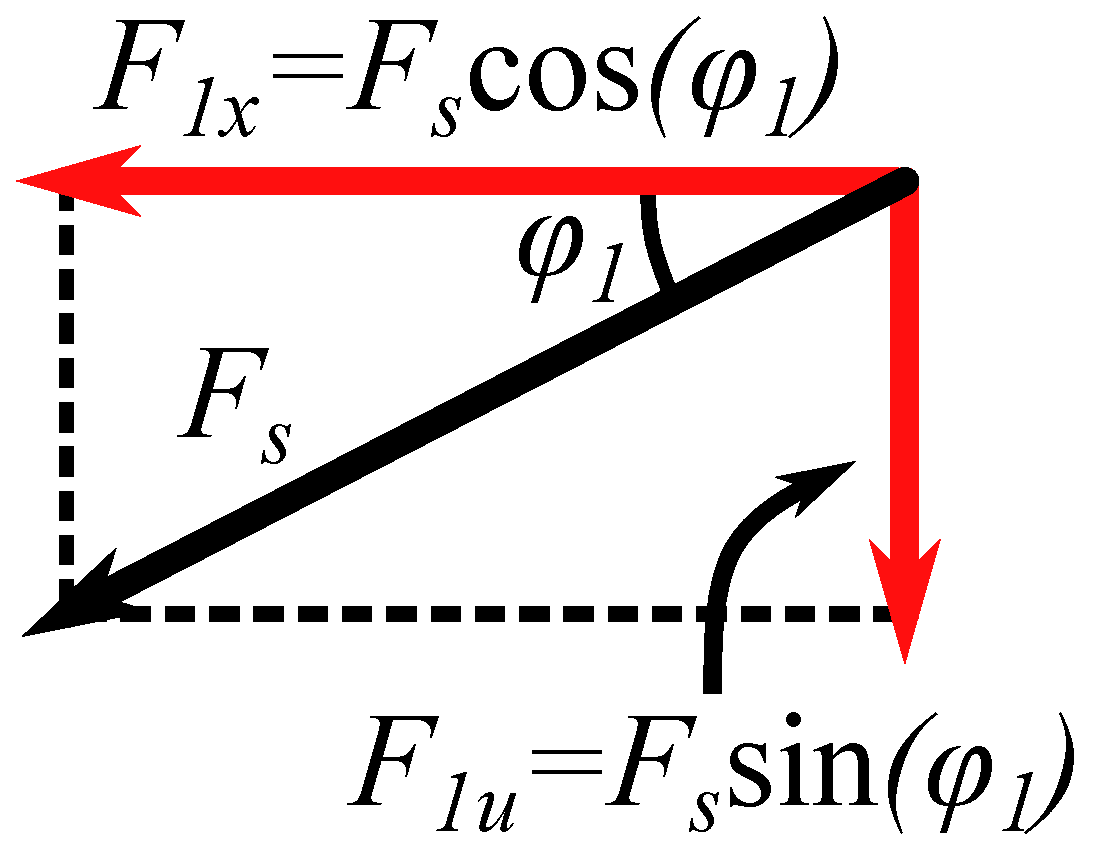
\includegraphics[width=\columnwidth]{Akustik/fig/force.eps}
    \end{subfigure}
    \caption{Fortegnet illustration af et delelement af snoren, samt de kræfter der virker på det, til venstre. Til højre er vist hvordan kraften kan opdeles i komponenter vha. trigonometri.}
    \label{aku:fig:string_forces}
\end{figure}
%
\subsection{Snorkræfter i kontinuitetsgrænsen}
For at bestemme kræften på delelementet af snoren betragtes \cref{aku:fig:string_forces}, hvor kraften i hver retning og ende af delelementet er tegnet som røde pile. Strengene på rigtige musikinstrumenter vibrerer aldrig ret meget sammenlignet med snorens længde -- $u(x,t) \ll L$ for alle $x$ og $t$. Det antages derfor at vinklerne i figuren $\phi_i \ll \nicefrac{\pi}{2}$. Alle kræfterne er snorkræfter\footnote{Her ses bort fra tyngdekraften, da den er den samme alle steder på snoren, og derfor kun påvirker snores placering i rummet, men ikke vibrationerne, der giver lyden.} og man kan vha. trigonometri, \cref{mat:eq:trig}, vise at
%
\begin{subequations} \label{aku:eq:string_force}
\begin{align}
    F_{1x} &= F_s\cos(\phi_1), \\
    F_{1u} &= F_s\sin(\phi_1), \\
    F_{2x} &= F_s\cos(\phi_2) = F_s\cos(\phi_1+\Delta\phi), \\
    F_{2u} &= F_s\sin(\phi_2) = F_s\cos(\phi_1+\Delta\phi).
\end{align}
\end{subequations}
%
Her er $\Delta \phi = \phi_2 - \phi_1$, og da delelementet er infinitesimalt, er størrelsen af snorkraften i begge ender den samme og kaldes $F_s$. For at få en differentialligning, vi har en chance for at løse, så er vi nød til at indføre en approksimation af kræfterne, hvilket er en smule teknisk og abstrakt, så læseren er velkommen til at tage resultatet,
%
\begin{align}
    F_x = F_{2x} - F_{1x} \simeq 0 \enspace , \enspace F_u = F_{2u} - F_{1u} \simeq F_s\Delta\phi,
\end{align}
%
for gode varer, og springe den følgende udledning over. \\

Da $\Delta\phi$ er infinitesimal giver det mening at rækkeudvikle til første orden omkring $\phi_1$ -- dvs. den variabel, der rækkeudvikles mht. er $\Delta\phi$. En funktions Taylorrække afhænger af den afledede, hvorfor disse bestemmes\footnote{Her betyder notationen $|_{\Delta\phi=0}$ at $\Delta\phi$ skal sættes lig med 0 efter funktionen er differentieret ligesom \cref{mat:eq:diff_eval} og analogt til klammenotationen i integralregning, \cref{mat:eq:klammestamfunktion}.}
%
\begin{align}
    \left.\dv{\cos(\phi_1+\Delta\phi)}{(\Delta\phi)}\right|_{\Delta\phi=0} &= \Big[-\sin(\phi_1+\Delta\phi)\Big]_{\Delta\phi=0} = -\sin(\phi_1), \\
    \left.\dv{\sin(\phi_1+\Delta\phi)}{(\Delta\phi)}\right|_{\Delta\phi=0} &= \Big[\cos(\phi_1+\Delta\phi)\Big]_{\Delta\phi=0} = \cos(\phi_1).
\end{align}
%
Nu kan \cref{mat:eq:Taylor_pol} bruges til at bestemme Taylorrækkerne for sinus og cosinus til første orden omkring $\phi_1$,
%
\begin{align}
    \cos(\phi_1+\Delta\phi) &\simeq \Big[\cos(\phi_1+\Delta\phi)\Big]_{\Delta\phi=0} + \Delta\phi\left.\dv{\cos(\phi_1+\Delta\phi)}{(\Delta\phi)}\right|_{\Delta\phi=0} = \cos(\phi_1) - \sin(\phi_1)\Delta\phi, \label{aku:eq:cos_taylor}\\
    \sin(\phi_1+\Delta\phi) &\simeq \Big[\sin(\phi_1+\Delta\phi)\Big]_{\Delta\phi=0} + \Delta\phi\left.\dv{\sin(\phi_1+\Delta\phi)}{(\Delta\phi)}\right|_{\Delta\phi=0} = \sin(\phi_1) + \cos(\phi_1)\Delta\phi. \label{aku:eq:sin_taylor}
\end{align}
%
Indsættes \cref{aku:eq:cos_taylor,aku:eq:sin_taylor} i \cref{aku:eq:string_force} fås
%
\begin{subequations}
\begin{align}
    F_{1x} &\simeq F_s\big[\cos(\phi_1) - \sin(\phi_1)\cdot0] = F_s\cos(\phi_1), \\
    F_{1u} &\simeq F_s\big[\sin(\phi_1) + \cos(\phi_1)\cdot0\big] = F_s\sin(\phi_1), \\
    F_{2x} &\simeq F_s\Big[\cos(\phi_1) - \sin(\phi_1)\Delta\phi], \\
    F_{2u} &\simeq F_s\Big[\sin(\phi_1) + \cos(\phi_1)\Delta\phi\Big].
\end{align}
\end{subequations}
%
Da kraften i både $F_{1x}$ og $F_{1u}$ peger i negativ retning, se \cref{aku:fig:string_forces}, er den totale kraft i henholdsvis $x$- og $u$-retningen på snorelementet
%
\begin{subequations} \label{aku:eq:f}
\begin{align}
    F_x &= F_{2x} - F_{1x} \simeq F_s\sin(\phi_1)\Delta\phi \simeq 0, \label{aku:eq:fx}\\
    F_u &= F_{2u} - F_{1u} \simeq F_s\cos(\phi_1)\Delta\phi \simeq F_s\Delta\phi. \label{aku:eq:fu}
\end{align}
\end{subequations}
%
Det sidste kommer af at $\phi_1$ per antagelse er et lille tal\footnote{Faktisk er dette helt stringent, idet vi rækkeudviklede til første orden. Idet $\phi_1$ også er et lille tal, så indeholder $\cos(\phi_1)\Delta\phi$ og $\sin(\phi_1)\Delta\phi$ både første og andenordensled, hvor orden nu hentyder til både $\phi_1$ og $\Delta\phi$, da begge tal er små. For at få en konsistent approksimation, skal vi således rækkeudvikle sinus og cosinus til første orden og se bort fra alle andenordensled. Da $\Delta\phi$ i sig selv er første orden, må vi kun beholde nulteordensledet i $\phi_1$, da vi ellers vil få noget af anden orden. Nulteordensledet i Taylorrækken for hhv. sinus og cosinus er $\sin(x)\simeq\sin(0)=0$ og $\cos(x)\simeq\cos(0)=1$.}, hvorfor $\sin(\phi_1) \simeq 0$ og $\cos(\phi_1)\simeq 1$. Ligning \eqref{aku:eq:f} er hvad man kalder den laveste ordens approksimation af kraften på snorelementet, hvilket giver den simpleste beskrivelse, og det viser sig at denne beskrivelse er særdeles god. \\

\subsection{Bølgeligningen}
Kombineres \cref{aku:eq:n2_kin,aku:eq:fu} gennem Newtons anden lov, der her gælder, fordi der betragtes et delelement af snores, fås
%
\begin{align} \label{aku:eq:n2_kont}
    \mu \pdv[2]{u(x,t)}{t} = F_s\frac{\Delta\phi}{\Delta x}.
\end{align}
%
Nu tage grænseværdien for $\Delta x \rightarrow 0$ af \cref{aku:eq:n2_kont}, hvor det bemærkes at venstresiden er uafhængig af $\Delta x$,
%
\begin{align} \label{aku:eq:n2_kont_2}
    \mu \pdv[2]{u(x,t)}{t} = \lim_{\Delta x\rightarrow0}F_s\frac{\Delta\phi}{\Delta x} = F_s\pdv{\phi}{x}.
\end{align}
%
Det sidste lighedstegn følger af definitionen på differentialkvotienten, \cref{mat:eq:diffkvotient}, hvor der dog fås partielt afledede, da $\phi$ er en funktion af to variable $t$ og $x$. Differentialkvotienten blev indført som hældningen på grafen for en funktion, og da $\phi$ er snorens hældning, så er $\phi = \nicefrac{\partial{u}}{\partial{x}}$. Indsættes dette i \cref{aku:eq:n2_kont_2} fås
%
\begin{align} \label{aku:eq:wave_eq}
    \pdv[2]{u(x,t)}{t} = \frac{F_s}{\mu} \pdv{}{x}\left(\pdv{u(x,t)}{x}\right) = \frac{F_s}{\mu} \pdv[2]{u(x,t)}{x},
\end{align}
%
hvilket netop er bølgeligningen, \cref{aku:eq:wave}, med $v_\mathrm{lyd}=\sqrt{\nicefrac{F_s}{\mu}}$. Vi har således vist at den simpleste model af en strengsvibrationer er løsningerne til bølgeligningen, og når strengen vibrerer skubber den til luften omkring den, hvorved den overfører sine vibrationer til trykbølger i luften. Man kan vise at andre instrumenter også producerer trykbølger beskrevet ved bølgeligningen, så den gælder ikke kun for strenginstrumenter.